%
% loesung.tex -- Beispiel-File für die Beschreibung der Loesung
%
% (c) 2020 Prof Dr Andreas Müller, Hochschule Rapperswil
%
\section{Anwendungen
\label{pade:section:Anwendungen}}
\rhead{Anwendungen}

In diesem Abschnitt werden ein paar Anwendungsmöglichkeiten der Padé-Approximation gezeigt.



\subsection{Totzeit Approximation
\label{pade:subsection:totzeit}}

In der Elektrotechnik werden des öfteren mathematische Probleme im Frequenzbereich gelöst, da dies oft einfacher zu berechnen ist.
Bei der Totzeit spricht man von einer Verzögerung im Zeitbereich, welche zum Beispiel in einem Regelkreis vorkommen kann.
Solche lineare zeitinvariante (LZI) Systeme oder besser bekannt unter dem englischen Begriff linear time-invariant (LTI) system, sind unabhängig von zeitlichen Verschiebungen. 
Jeder, der sich mit LTI Systemen auseinander gesetzt hat, weiss, dass eine Totzeit $T$ im Frequenzbereich
\begin{equation*}
H(s) = e^{-sT}
\end{equation*}
durch eine Exponentialfunktion ausgedrückt wird.
Verschiedene Methoden wie z.B. die Wurzelortskurven, können nicht mit Totzeiten umgehen, sondern nur mit Übertragungsfunktionen, welche als gebrochen rationale Funktionen vorliegen.
Weshalb die Übertragungsfunktion eines Systems typischerweise als gebrochene Polynome, eine Form welche einer rationalen Funktion
\begin{equation*}
H(s)=\frac{P(s)}{Q(s)}
\end{equation*}
entspricht, vorkommt.
Diese gebrochenen Polynome verwendet man, um Pol- und Nullstellen zu finden und damit weitere Analysen durchzuführen. 
Mit $e^{-sT}$ haben wir jedoch keine brauchbaren Pol- Nullstellen welche wir analysieren können.
Dies kann jedoch gefordert sein, wenn man eine zeit kontinuierliche Analyse machen möchte.
Eine Lösung dafür könnte nun sein, $e^{-sT}$ zu approximieren und die Approximation für weitere Rechnungen zu verwenden.
Die Padé-Approximation der Exponentialfunktion ist glücklicherweise schon sehr gut bekannt und kann mit den Formeln \ref{pade:expP} und \ref{pade:expQ} für eine beliebig hohe Ordnung ermittelt werden.

Die Qualität dieser Approximation können wir nun in einer logarithmischen Skala mit der originalen Funktion vergleichen.
In der Grafik \ref{pade:totzeitexp} ist ersichtlich das die Padé-Approximation mit steigendem Grad bessere Resultate liefert und sich der Exponentialfunktion mehr und mehr annähert.

\begin{figure}[!h]
	\centering
	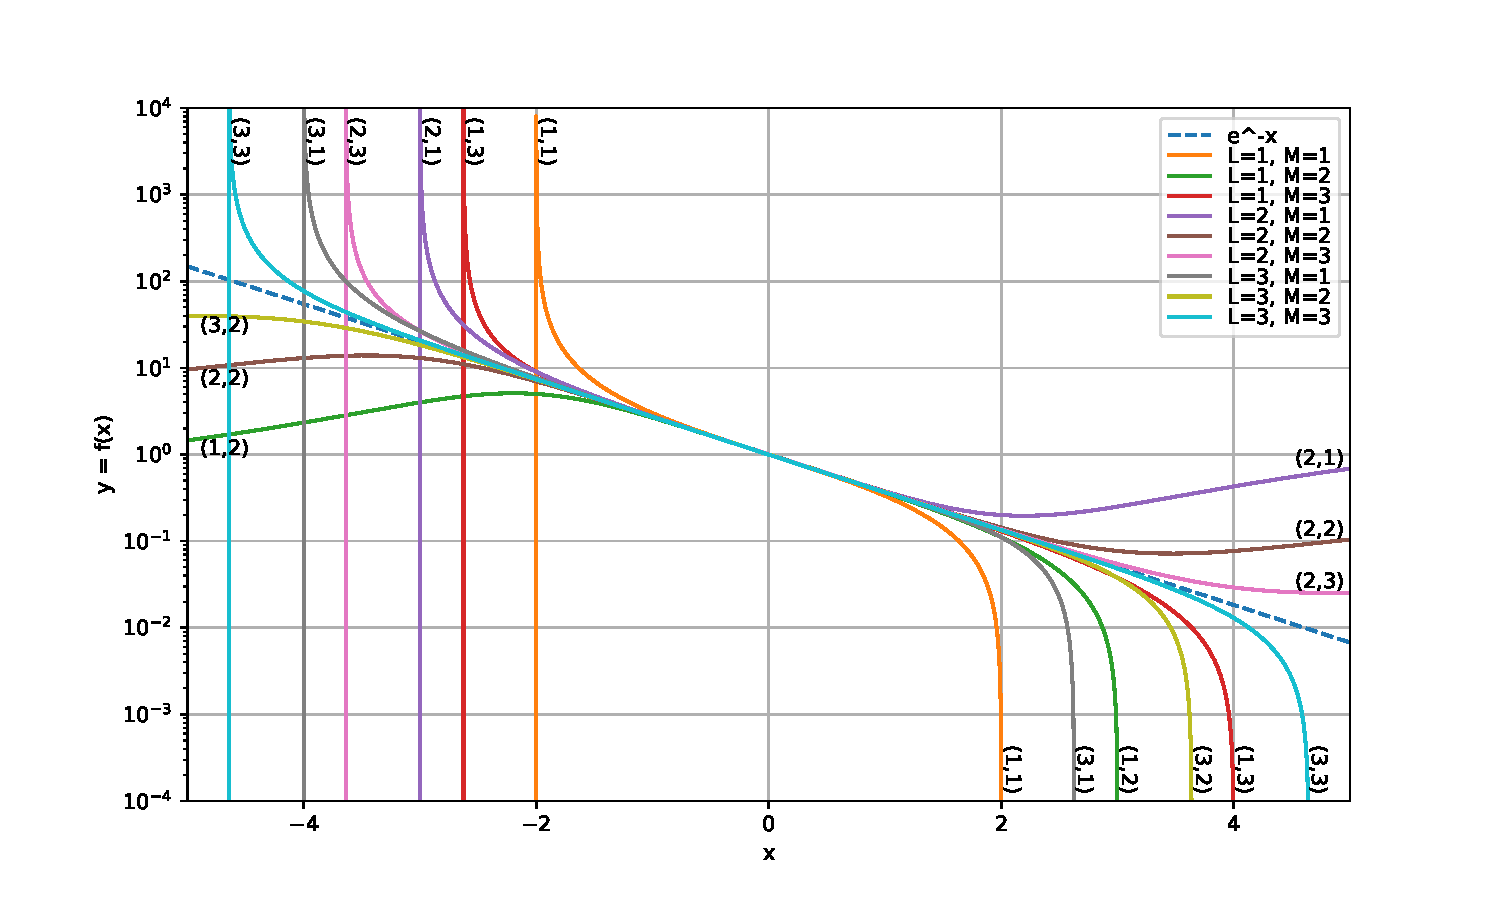
\includegraphics[width=1\linewidth]{./papers/pade/python/bilder/totzeit.pdf}
	\caption{Plot der Padé-Approximanten der Exponentialfunktion im Vergleich zu der Originalfunktion in einer logarithmischen Skala vergleichend mit der Taylorreihe sechster Ordnung der Exponentialfunktion.\label{pade:totzeitexp}}
\end{figure}

Die Grade werden dabei im Nenner und Zähler unterteilt aufgezeigt.
In diesem Beispiel \ref{pade:totzeitexp} mit der Exponentialfunktion erweisen sich die Polynome des selben Grades im Nenner und Zähler als die geeignetsten.
Wobei mit steigendem Grad eine stetige Verbesserung zugrunde liegt.
Zum Vergleich wurde noch die Taylorreihe von $e^{-x}$ der sechsten Ordnung in der Grafik \ref{pade:totzeitexp} dargestellt. 
Diese ist im negativen Bereich der Funktionsachse deutlich schlechter als die Padé-Approximanten, jedoch verhält sie sich im positiven Bereich besser.


Nehmen wir nun diese Polynome, welche sich noch im Frequenzbereich befinden und transformieren diese wieder zurück in den Zeitbereich, erhalten wir die in der Grafik dargestellten \ref{pade:totzeitexp2} Kurven.

\begin{figure}[!h]
	\centering
	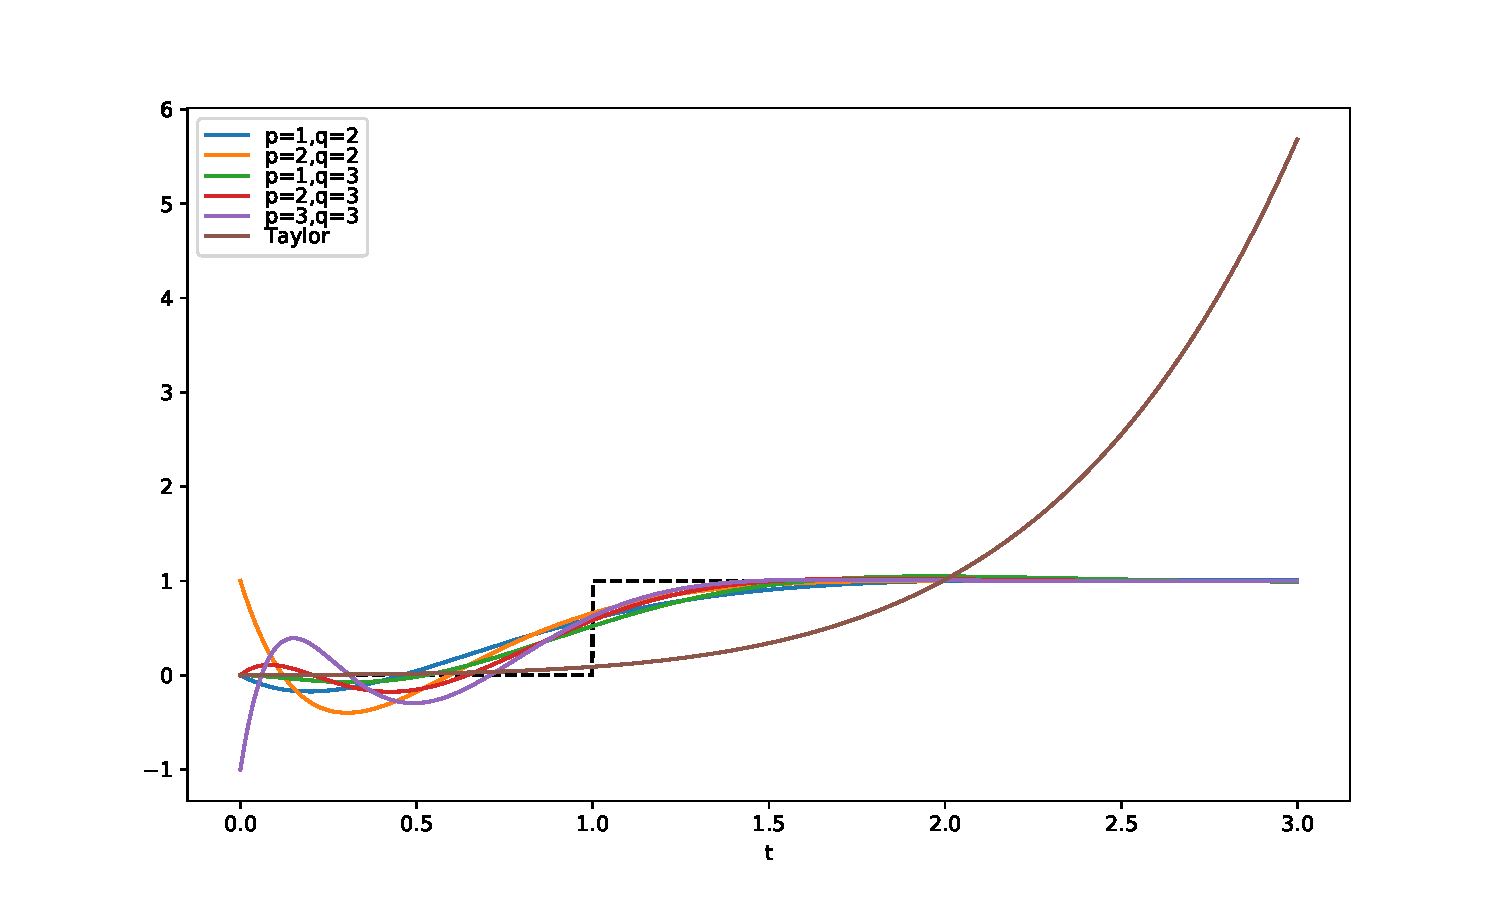
\includegraphics[width=1\linewidth]{./papers/pade/python/bilder/padelow33.pdf}
	\caption{In den Zeitbereich zurück transformierte Polynome tieferer Ordnung\label{pade:totzeitexp2}.}
\end{figure}

Die Polynome unterer Ordnung sind dabei noch weit von einem brauchbaren Ergebnis des gesuchten verzögerten Einheitssprunges entfernt.
Man kann nun die Ordnung der Polynome weiter erhöhen bis man eine zufriedenstellende Approximation erhält.
Dabei muss man jedoch aufpassen welche Methode für die Rücktransformation verwendet wird.
Nicht alle Implementationen der Rücktransformation von Übertragungsfunktionen in ein Zustandsraummodell sind nummerisch stabil. 
Bei Polynomen grosser Ordnung oder wenn das Nenner- und Zählerpolynom nicht gleicher Ordnung sind, können bei einer Rücktarnformation Fehler auftauchen.
Dies ist jedoch ein anderes Thema welches den Rahmen dieses Papers sprengen würde und wird deshalb nicht weiter beschrieben.


\begin{figure}[h]
	\centering
	\subfigure[Pole und Nullstellen im Bildbereich geplottet wenn $P=Q$ ist.\label{pade:poles1}]{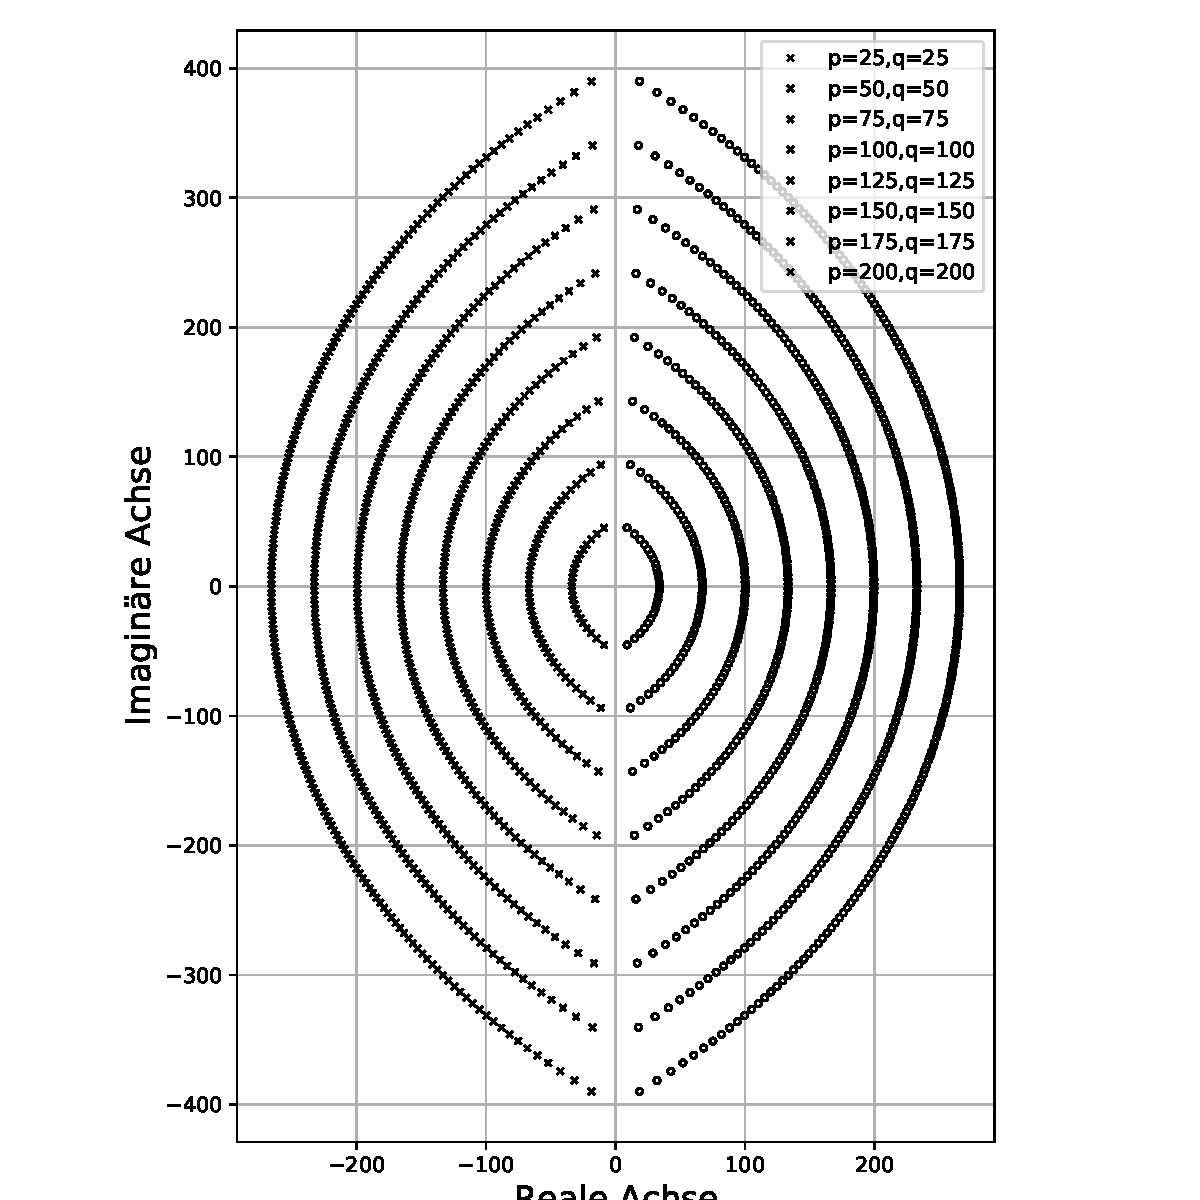
\includegraphics[width=0.40\linewidth]{./papers/pade/python/bilder/poles1.pdf}}
	\subfigure[Pole und Nullstellen im Bildbereich geplottet wenn $P>Q$ ist.\label{pade:poles2}]{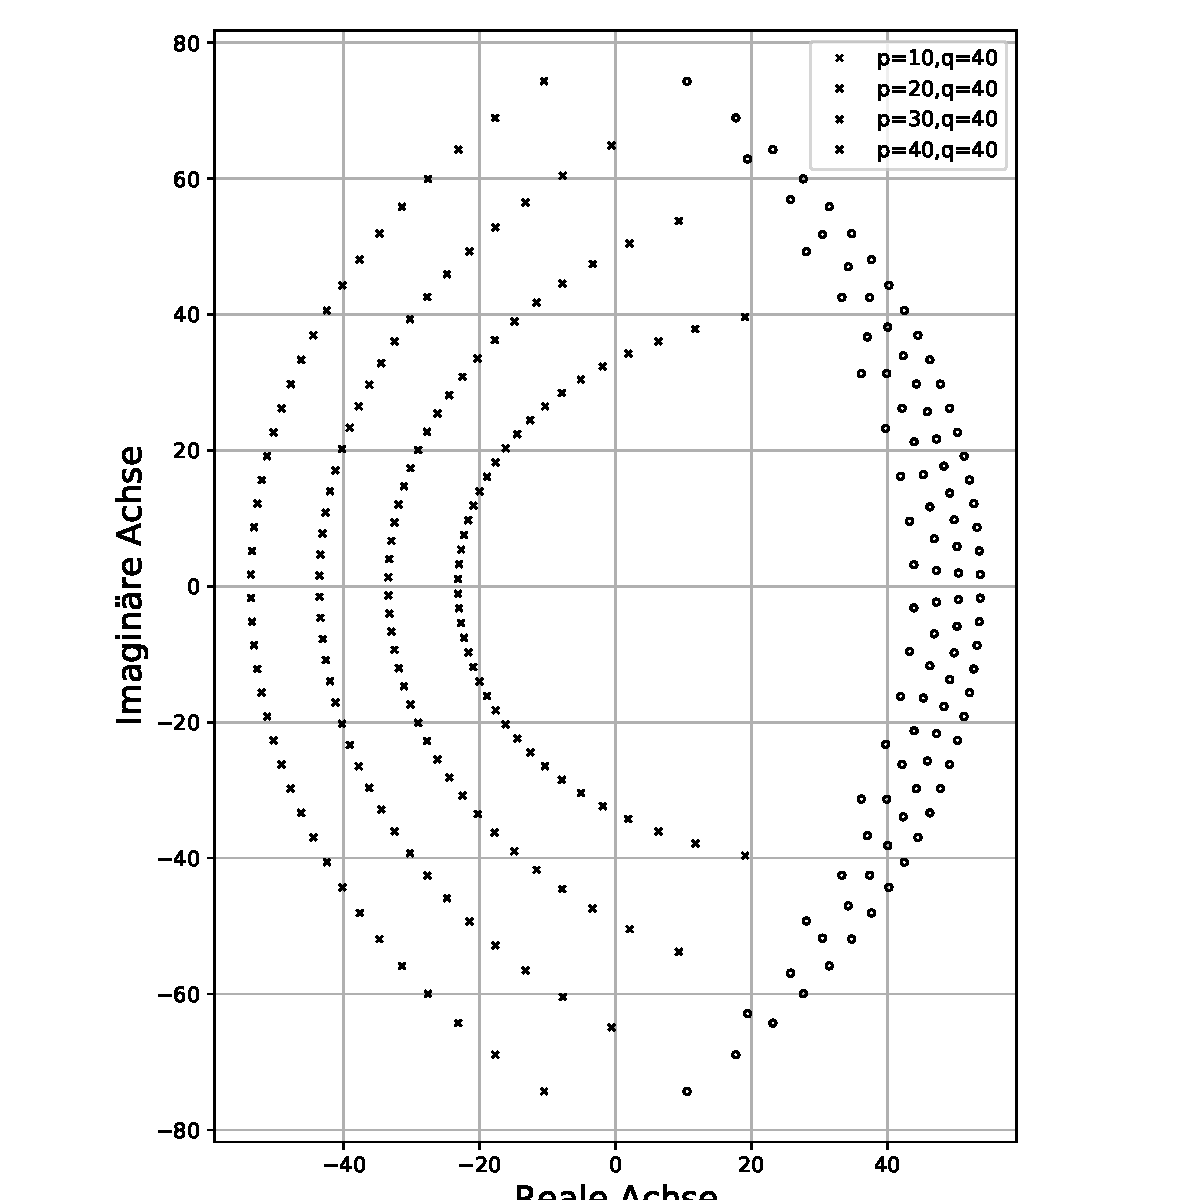
\includegraphics[width=0.40\linewidth]{./papers/pade/python/bilder/poles2.pdf}}
	\subfigure[Pole und Nullstellen im Bildbereich geplottet wenn $P<Q$ ist.\label{pade:poles3}]{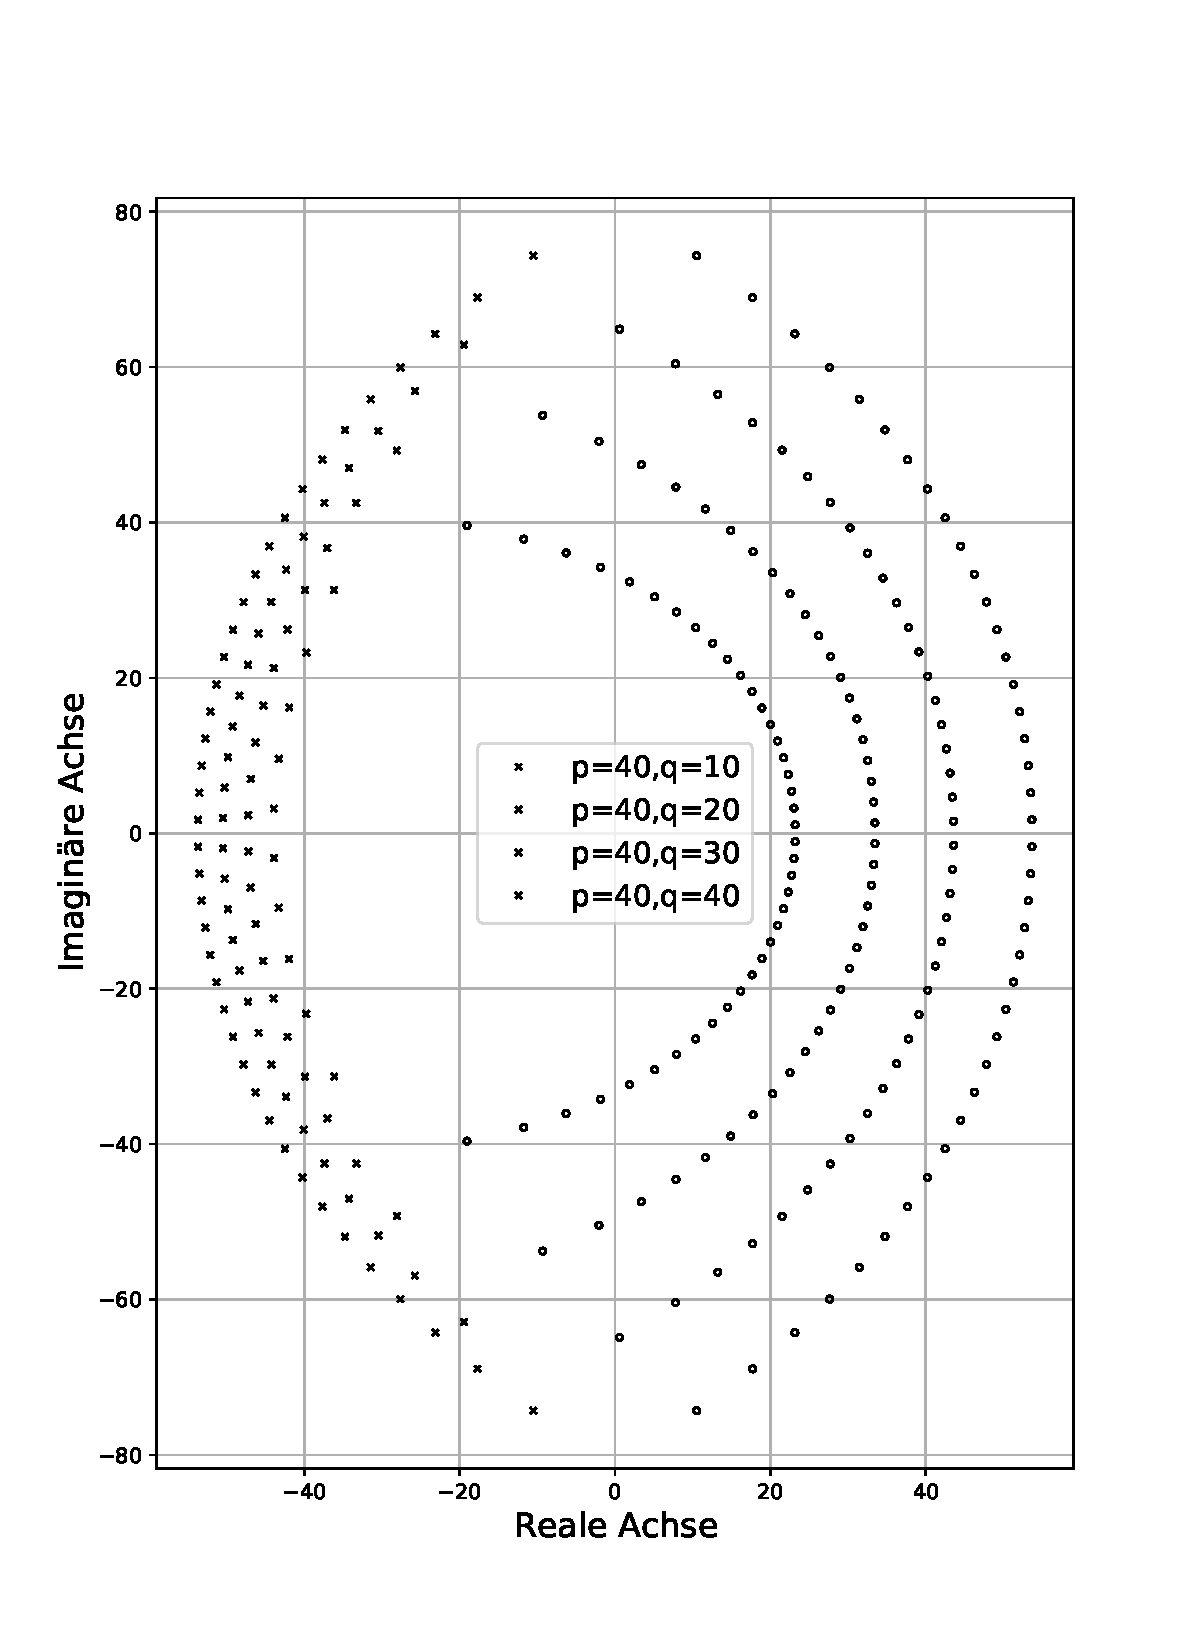
\includegraphics[width=0.40\linewidth]{./papers/pade/python/bilder/poles3.pdf}}
	\caption{Visualisierung der Stabilität der Padé-Polynome bei ungleicher $[L/M]$ Ordnung. \label{pade:prole}}
\end{figure}

In der Grafik \ref{pade:prole} sind nun die Pol- und Nullstellen von höheren Ordnungen dargestellt. 
Auffallend ist die schöne Symmetrie der Pole und Nullstellen welche bei gleicher Ordnung der Nenner- und Zählerpolynome um den Nullpunkt verteilt sind.
Diese Symmetrie verschwindet wenn der Grad des Nenner oder des Zählerpolynoms grösser gewählt wird.
Dies kann man soweit treiben bis eine die Polstellen in den rechten Bereich der komplexen Ebene reichen \ref{pade:poles2},
was ein instabiles System zur folge hat.
Ein instabiles System beutetet hier, dass der rücktransformierte Einheitssprung eine immer grösser werdende Schwingung ist.
 
\begin{figure}
	\centering
	\subfigure[Pole und Nullstellen im Bildbereich geplottet wenn $P=Q$ ist.\label{pade:totzeit1}]{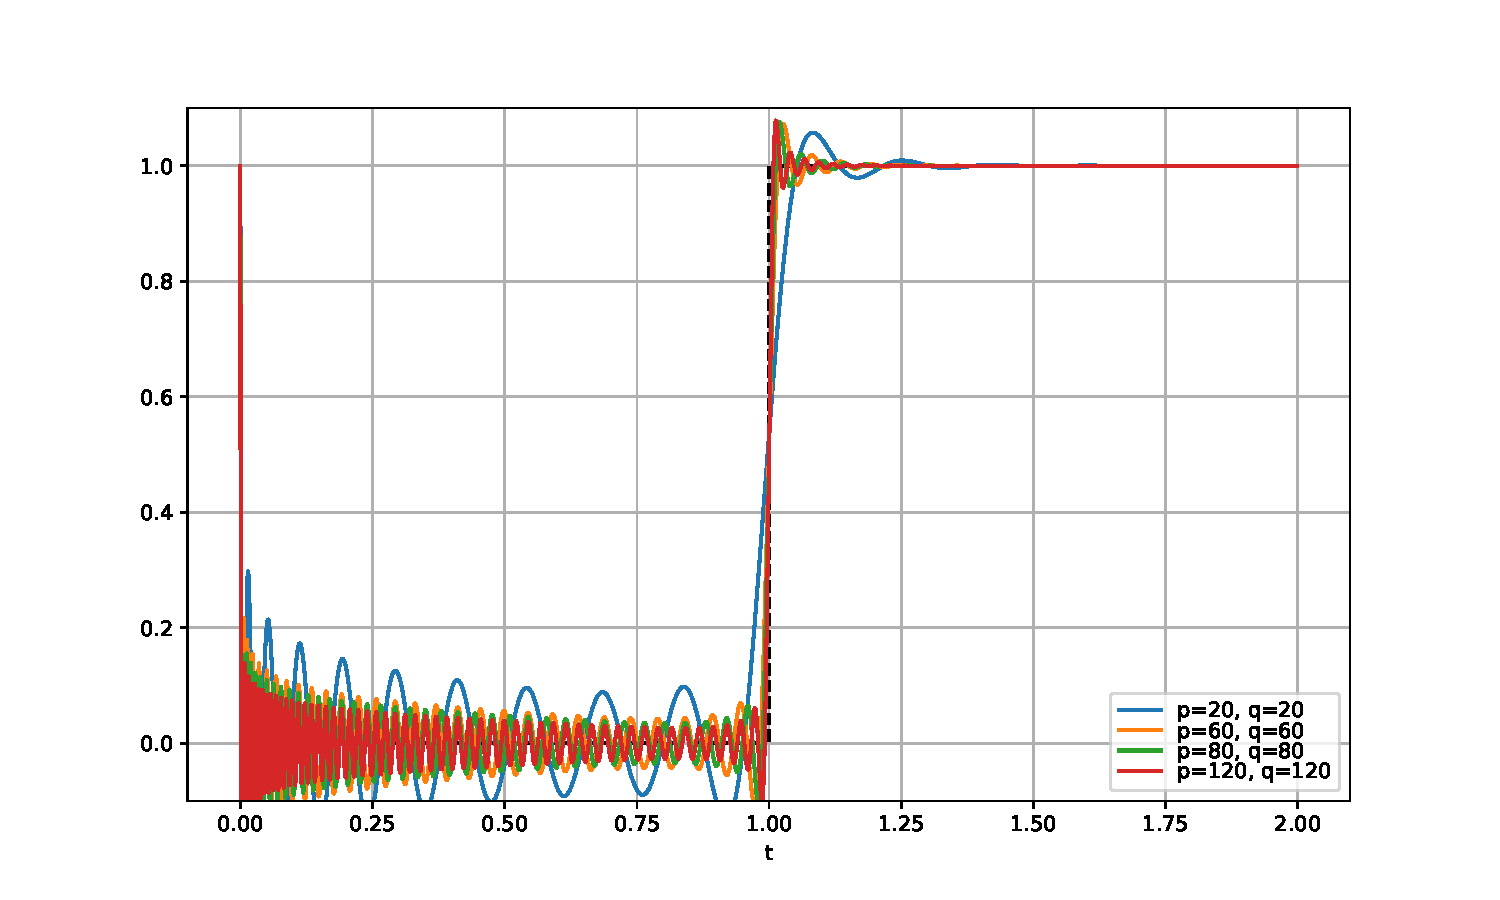
\includegraphics[width=1\linewidth]{./papers/pade/python/bilder/padehigh1.pdf}}
	\subfigure[Pole und Nullstellen im Bildbereich geplottet wenn $P=Q-10$ ist.\label{pade:totzeit2}]{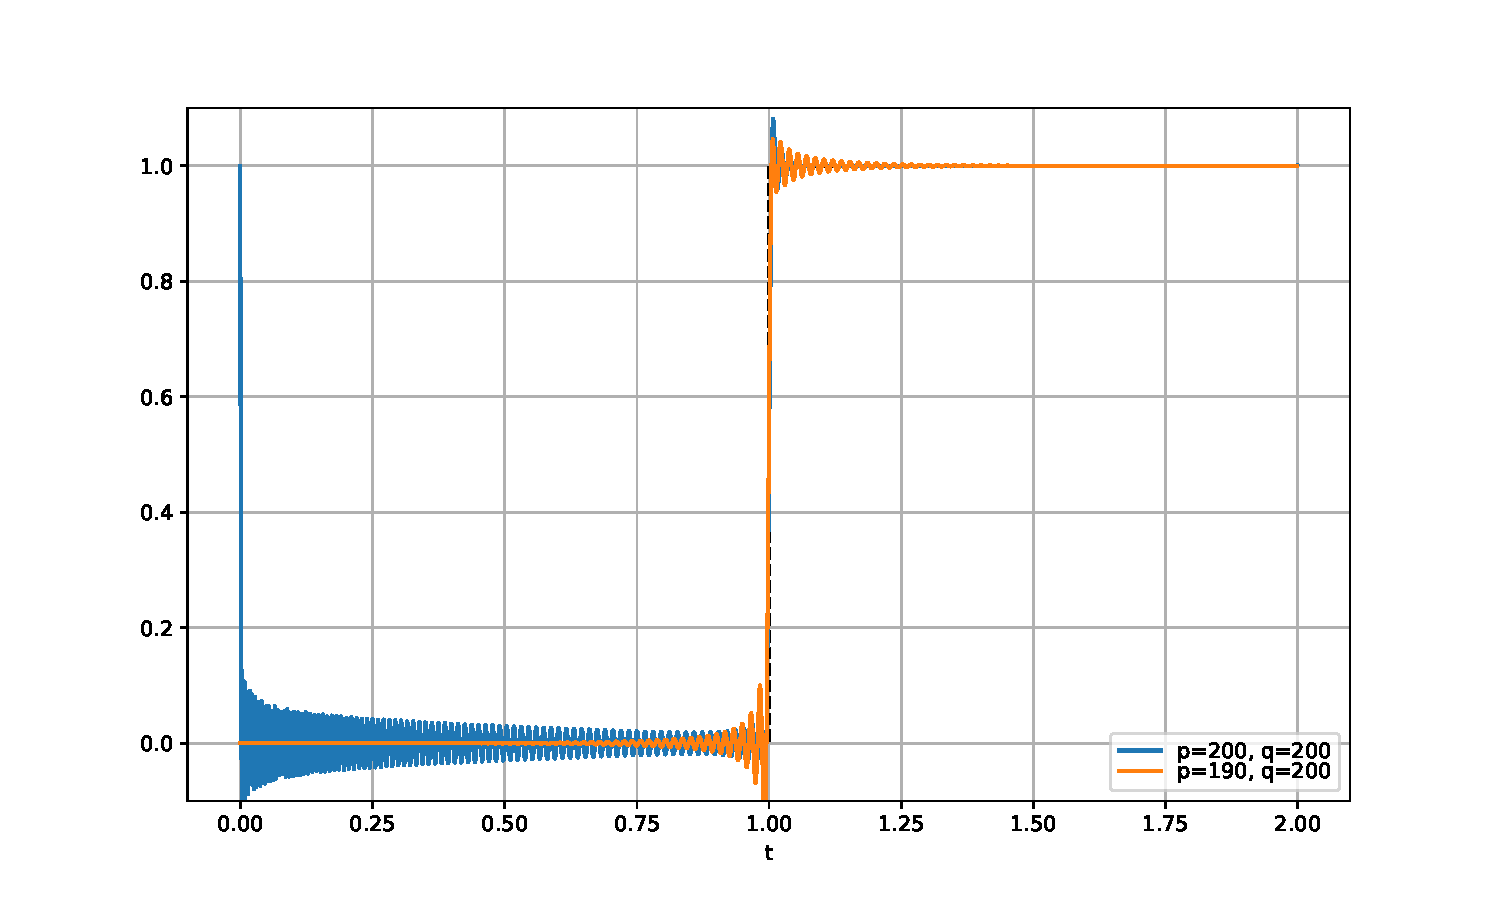
\includegraphics[width=1\linewidth]{./papers/pade/python/bilder/padehigh2.pdf}}
\end{figure}
Verwendet man nun die Approximanten höheren und gleicher Ordnung für die Rücktransformation in Grafik \ref{pade:totzeit1}, erhält man einen immer besser werdenden Einheitssprung mit einem kleinen Überschwinger vor und nach dem Sprung. 
Auffallend ist hier das der Padé-Approximant höchster Ordnung zu beginn den grössten Fehlerpeak hat.
Dieser ist sogar so hoch wie der Einheitssprung selbst.

Um diesen Fehlerpeak zu beginn ein wenig zu vermindern können nun die Pole in der komplexen Ebene ein wenig näher zur positiven Halbebene gebracht werden.
Wie schon in  dem Pol- Nullstellendiagramm \ref{pade:poles2} erkennbar ist das mit einer Differenz von der Ordnung des Zählerpolynoms $p$ und Nennerpolynom $q$ möglich.
Mit einer Differenz von 190 zu 200 der Polynom Ordnung, wurde die Rücktransformierte des Padé-Approximanten der Grafik \ref{pade:totzeit2} dargestellt.
Deutlich zu sehen ist dabei, dass der Überschwinger welcher bei dem Padé-Approximanten gleicher Ordnung in derselben Grafik \ref{pade:totzeit2} nocher vorhanden ist, verschwindet.
Jedoch besitzt der Approximant ungleicher Ordnung eine längere Einschwingzeit als die der gleicher Ordnung. 
Mit diesen Werten der Ordnungen kann in der Praxis solange Optimiert werden bis man die beste Lösung für sein Problem gefunden hat.
Es gäbe dabei noch die Möglichkeit weitere Filter einzubauen um diese Schwingungen zu dämpfen und ein noch besseres Resultat zu erzielen.


\newpage

\subsection{Signal Modellierung
	\label{pade:subsection:SignalMod}}

Das Ziel einer Signalmodellierung ist dass eine parametrische Beschreibung eines Signales gefunden wird.
Dies kann für die Filterentwicklung, Interpolation, Extrapolation oder Kompression verwendet werden.
Dabei kann man immer das gleiche Modell verwenden, welches der Ausgang eines linearen verschiebungsinvarianten Filters zu einem Eingang $v(n)$ darstellt. 
\begin{center}
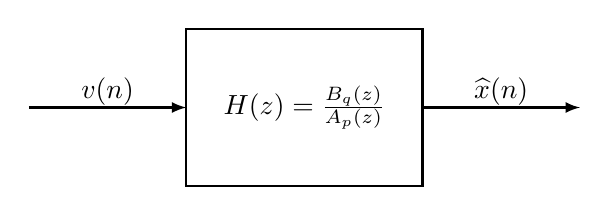
\begin{tikzpicture}
\tikzset{>=latex}
\node at (-1,1.2)  {$v(n)$}; 
\draw[thick,->] (-2,1)--(0,1);
\draw[thick] (0,0) rectangle (3,2) node[pos=.5] {$H(z)=\frac{B_q (z)}{A_p (z)}$};
\draw[thick,->] (3,1)--(5,1);
\node at (4,1.2)  {$\widehat{x}(n)$}; 
\end{tikzpicture}
\end{center}
Dieses Modell wird mit

\begin{equation}
H(z)
=
\frac{B_{q}(z)}{A_{p}(z)}
=
\frac{\sum_{k=0}^{q} b_{q}(k) z^{-k}}{1+\sum_{k=1}^{p} a_{p}(k) z^{-k}}
\end{equation}
als eine rationale Funktion beschrieben.
Das Eingangssignal welches auf den Filter wirkt ist meist ein diskreter Impuls $\delta(n)$.
Der Modellierungsfehler $e^{\prime}(n)$ setzt sich dabei aus der Differenz der Einheitssprungantwort $h(n)$ und dem diskreten Signal $x(n)$ zusammen.
\begin{center}
	\tikzset{>=latex}
	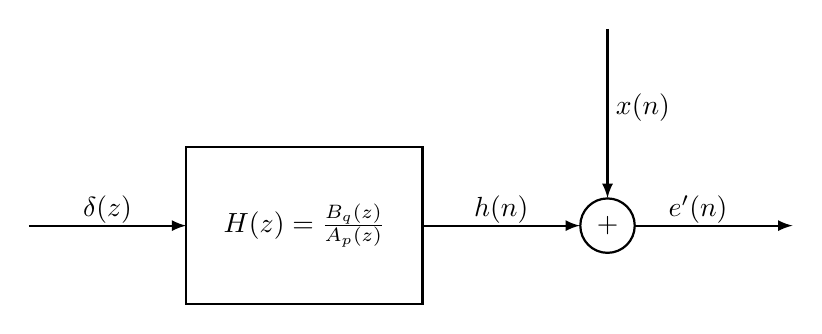
\begin{tikzpicture}
	\node at (-1,1.2)  {$\delta(z)$}; 
	\draw[thick,->] (-2,1)--(0,1);
	\draw[thick] (0,0) rectangle (3,2) node[pos=.5] {$H(z)=\frac{B_q (z)}{A_p (z)}$};
	\draw[thick,->] (3,1)--(5,1);
	\node [circle, draw, thick] at (5.35,1){+};
	\draw[thick,->] (5.35,3.5)--(5.35,1.35);
	\draw[thick,->] (5.7,1)--(7.7,1);
	\node at (4,1.2)  {$h(n)$}; 
	\node at (5.8,2.5)  {$x(n)$}; 
	\node at (6.5,1.2)  {$e^{\prime}(n)$}; 
	\end{tikzpicture}
\end{center}
Dabei ist das Ziel den quadratischen Fehler (Least Squares Method)
\begin{equation}
E_{L S}
=
\sum_{n=0}^{\infty}\left|e^{\prime}(n)\right|^{2}
\end{equation}
des Systems zu minimieren.
Um dies zu erreichen   
\begin{equation}\begin{array}{ll}
\frac{\partial E_{L S}}{\partial a_{p}^{*}(k)}
=
0 
& 
\text{mit } k=1,2, \ldots, p \\
&\\

\frac{\partial E_{L S}}{\partial b_{q}^{*}(k)}
=
0  
&
 \text{mit } k=0,1, \ldots, q
\end{array}\end{equation}
werden die Ableitungen gleich 0 gesetzt.
Aus diesen Bedienungen resultiert eine Menge von nichtlinearen Gleichungen 

\begin{equation}
\frac{\partial E_{L S}}{\partial a_{p}^{*}(k)}
=
\frac{1}{2 \pi} 
\int_{-\pi}^{\pi}
\left[X\left(e^{j \omega}\right)-\frac{B_{q}\left(e^{j \omega}\right)}{A_{p}\left(e^{j \omega}\right)}\right] 
\frac{B_{q}^{*}\left(e^{j \omega}\right)}{A_{p}^{*}\left(e^{j \omega}\right)^{2}} 
e^{j k \omega} d \omega
=
0
\end{equation}
\begin{equation}
\frac{\partial E_{L S}}{\partial b_{q}^{*}(k)}
=
-\frac{1}{2 \pi} 
\int_{-\pi}^{\pi}
\left[X\left(e^{j \omega}\right)-\frac{B_{q}\left(e^{j \omega}\right)}{A_{p}\left(e^{j \omega}\right)}\right] 
\frac{e^{j k \omega}}{A_{p}^{*}\left(e^{j \omega}\right)} d \omega
=
0
\end{equation}

welche möglicherweise sehr schwierig lösbar sind.
Aus diesem Grund wird in der Praxis der Ansatz des kleinsten quadratischen Fehlers vermieden. 
Um diese nichtlinearen Gleichungen zu vermeiden und dennoch eine Lösung zu finden, welche uns ein passende Nummer von $x[n]$ Werten mit der Einheitssprungantwort verbindet, kann ein eleganter Trick 
\begin{equation}
H(z) A_{p}(z)=B_{q}(z)
\end{equation}
verwendend werden. 
In der Zeitebene betrachtet
\begin{equation}
h(n)+\sum_{k=1}^{p} a_{p}(k) h(n-k)=b_{q}(n)
\end{equation}
handelt es sich in bei dieser Gleichung um eine Faltung.
Wobei die rechte Seite der Gleichung für $n>q$ gleich null ist.
Diese Fallunterscheidung
\begin{equation}
x(n)+\sum_{k=1}^{p} a_{p}(k) x(n-k)
=
\left\{\begin{array}{cc}
b_{q}(n) & 
\text{mit } \quad n=0,1, \ldots, q \\
0 & 
\quad\text{mit } \quad n=q+1, \ldots, q+p
\end{array}\right.\end{equation}
kann in eine matrix Form gebracht werden.
\begin{equation}
\left[\begin{array}{cccc}
x(0) & 0 & \cdots & 0 \\
x(1) & x(0) & \cdots & 0 \\
x(2) & x(1) & \cdots & 0 \\
\vdots & \vdots & & \vdots \\
x(q) & x(q-1) & \cdots & x(q-p) \\
x(q+1) & x(q) & \cdots & x(q-p+1) \\
\vdots & \vdots & & \vdots \\
x(q+p) & x(q+p-1) & \cdots & x(q)
\end{array}\right]
\left[\begin{array}{c}
1 \\
a_{p}(1) \\
a_{p}(2) \\
\vdots \\
a_{p}(p) \\
\end{array}\right]
=
\left[\begin{array}{c}
b_{q}(0) \\
b_{q}(1) \\
b_{q}(2) \\
\vdots \\
b_{q}(q) \\
0 \\
\vdots \\
0
\end{array}\right]
\end{equation}
Diese Matrix ist uns schon aus dem Abschnitt \ref{pade:subsection:Pade_erstellen} bekannt es handelt sich nämlich um eine Padé-Approximation.
Welche wir nun für das Signal mit einer vorgegebener Ordnung berechnen können.

\textbf{Beispiel:}

Die ersten sechs Signale eines Signales sind vorgegeben.
\begin{equation*}
\bm x=\left[
\begin{array}{l}
1.0000\\
1.5000\\
0.7500\\
0.3750\\
0.1875 \\
0.0938
\end{array}\right]
\end{equation*}
Das Ziel ist drei verschiedene Padé-Approximanten mit drei verschiedenen Freiheitsgraden zu finden.
\begin{equation*}\begin{aligned}
&\begin{array}{ll}
\text { All pole } & (q=0, p=2) \\
\text { FIR } & (q=2, p=0)\\
\text { IIR } &(\mathrm{q}=1, \mathrm{p}=1)
\end{array}\\
\end{aligned}\end{equation*}

Das All pole Modell $(q=0,p=2)$ wird in die Matrixform
\begin{equation}\left[\begin{array}{ccc}
x(0) & 0 & 0 \\
x(1) & x(0) & 0 \\
x(2) & x(1) & x(0)
\end{array}\right]\left[\begin{array}{c}
1 \\
a_1 \\
a_2
\end{array}\right]=\left[\begin{array}{c}
b_0 \\
0 \\
0
\end{array}\right]\end{equation}
gebracht. 
Von der ersten Gleichung folgt, dass der Wert $b_0 = x(0)=1$ ergeben muss. 
Weiter können nun die letzten zwei Gleichungen
\begin{equation}\left[\begin{array}{ll}
x(0) & 0 \\
x(1) & x(0)
\end{array}\right]\left[\begin{array}{l}
a_1 \\
a_2
\end{array}\right]=-\left[\begin{array}{l}
x(1) \\
x(2)
\end{array}\right]\end{equation}
eingesetzt und gelöst
\begin{equation}\left[\begin{array}{cc}
1 & 0 \\
1.5 & 1
\end{array}\right]\left[\begin{array}{l}
a_1 \\
a_2
\end{array}\right]=-\left[\begin{array}{c}
1.50 \\
0.75
\end{array}\right]\end{equation}
\begin{equation}
a_1=-1.50 \quad  \quad a_2=1.50
\end{equation}
werden.
Somit haben wir das Ergebnis für unser $x(n)$
\begin{equation}
H(z)=\frac{1}{1-1.50 z^{-1}+1.50 z^{-2}}
\end{equation}
berechnet.
Man sollte beachten, dass sich die Pole nicht im Einheitskreis befinden und somit das Resultat kein stabiles Modell sein wird.

Für das FIR-Modell $(q=2,P=0)$ ist das Resultat einfach
\begin{equation}\begin{array}{r}
A(z)=1 \\
{\left[\begin{array}{l}
	x(0) \\
	x(1) \\
	x(2)
	\end{array}\right]=\left[\begin{array}{l}
	b_0 \\
	b_1 \\
	b_2
	\end{array}\right]}
\end{array}\end{equation} 
berechenbar.
Somit erhalten wir 
\begin{equation}
H(z)=1+1.50 z^{-1}+0.75 z^{-2}
\end{equation}
als Modell.

Für das IIR-Modell mit $(q=1,p=1)$ welches die Form
\begin{equation}
H(z)=\frac{b(0)+b(1) z^{-1}}{1+a(1) z^{-1}}
\end{equation}
erhalten wird, sind die Padé-Gleichungen

\begin{equation}\left[\begin{array}{ll}
x(0) & 0 \\
x(1) & x(0) \\
x(2) & x(1)
\end{array}\right]\left[\begin{array}{c}
1 \\
a_1
\end{array}\right]=\left[\begin{array}{c}
b_0 \\
b_1\\
0
\end{array}\right]\end{equation}
woraus der Pol in der letzten Gleichung 
\begin{equation}
x(2)+a_1 x(1)=0
\end{equation}
gerechnet werden kann.
Einsetzt und nach $a_1$ Aufgelöst erhalten wir
\begin{equation}
a_1=-\frac{x(2)}{x(1)}=
-\frac{0.75}{1.5}=
-0.5
\end{equation}
Mit den bekannten Polen können nun die Nullstellen mit den oberen zwei Gleichungen 
\begin{equation}\left[\begin{array}{c}
b_0 \\
b_1
\end{array}\right]=\left[\begin{array}{cc}
1 & 0 \\
1.5 & 1
\end{array}\right]\left[\begin{array}{c}
1 \\
-0.5
\end{array}\right]=\left[\begin{array}{l}
1 \\
1
\end{array}\right]\end{equation}
gerechnet werden.
Die Koeffizienten können nun in das Modell eingesetzt werden, womit wir
\begin{equation}
H(z)=\frac{1+z^{-1}}{1-0.5 z^{-1}}
\end{equation}
erhalten.
Dieses Modell hat eine identische Einheitssprungantwort 
\begin{equation}
h(n)=(0.5)^{n} u(n)+(0.5)^{n-1} u(n-1)
=
\delta(n)+1.5(0.5)^{n-1} u(n-1)\end{equation}
wie $x(n)$.
Dies ist jedoch ein Spezialfall und kommt nicht immer vor.






